% !TeX root = ./descente_de_charge.tex % Pour compiler depuis ce fichier
% !BIB TS-program = biber

\documentclass{rSIMONIN} % Pour le modèle de rapport de stage de la SIMONIN

% Import des variables et infos générales du document
\import{latex_files/}{main_infos.tex} % Import des infos générales du document
% \client{HARING}
% \projet{Atrium La}
% \reference{ABN AMRO Atrium La}
% \editor{JB et Nico}
% \emaileditor{jbjournot@simonin.com}
% \numeroaffaire{2403-184}
% \numeroreference{ }
% \numerodoc{2404-500-03}

\begin{document}

\pagestyle{rSIMONIN} % Pour que notre document utilise ce style
\thispagestyle{empty} % Pour que la page de garde n'ait pas de numéro
\frontpageSTB % Pour le modèle rapports de Stages des Branches / Master

%%%%%%%%%%%%%%%%%%%%%%
%% Sommaire
%%%%%%%%%%%%%%%%%%%%%%
{
    \setcounter{tocdepth}{1} % Profondeur du sommaire
    \renewcommand{\contentsname}{Sommaire} % Nom du sommaire
    \tableofcontents % Affichage du sommaire
}
\clearpage % Pour forcer le sommaire à être sur une page seule


%%%%%%%%%%%%%%%%%%%%%%
%% INFORMATIONS GENERALES
%%%%%%%%%%%%%%%%%%%%%%
\newpage % Pour forcer le début d'une nouvelle page

\chapter{INFORMATIONS GENERALES} % Titre du chapitre

\section{Situation de l'ouvrage} % Titre de la section

Affaire/projet : \numeroaffaire \numeroreference  \\ % Affichage du numéro d'affaire 
Note d'hypothèse N° : \notehypotheses \\ % Affichage de la note d'hypothèse
Adresse: \adresseprojet \\ % Affichage de l'adresse du projet


\begin{figure}[H] % Pour insérer une figure
    \centering % Pour centrer l'image
    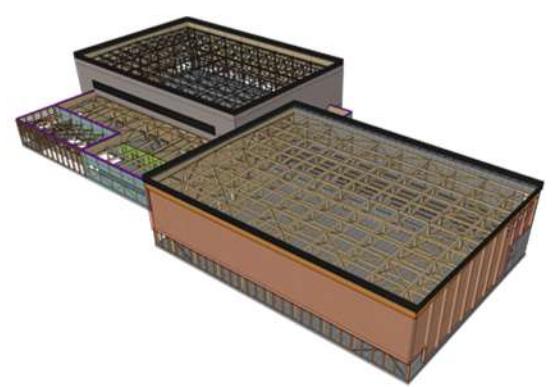
\includegraphics[width=0.7\textwidth]{input_data/situation_ouvrage.png} % Pour insérer l'image
    \caption{Description de l'ouvrage} % Légende de l'image
\end{figure}

\section{Plan de situation}

\section{Description de l'ouvrage}

\section{Règles de calcul et de conception}

Les calculs de structures sont réalisés conformément aux normes Eurocode en vigueur :
\begin{enumerate}
    \item Eurocode 0 EN 1990 : Base de calcul des structures
    \item Eurocode 1 EN 1991 : Actions sur les structures
    \item Eurocode 2 EN 1992 : Calculs des structures en béton
    \item Eurocode 3 EN 1993 : Calculs des structures en acier
    \item Eurocode 4 EN 1994 : Calculs des structures mixtes acier-béton
    \item Eurocode 5 EN 1995 : Calculs des structures en bois
    \item Eurocode 6 EN 1996 : Calculs des structures en maçonnerie
    \item Eurocode 8 EN 1998 : Calculs des structures pour leur résistance aux séismes
    \item Résix® Technique d assemblage sous avis technique CSTB 3.3-19-986 V1
\end{enumerate}




\section{Stabilité et Repérage des points d'appuis}
\subsection{Principe de stabilité de la structure}

\subsection{Repérage des points d'appuis}

\begin{figure}[H] % Pour insérer une figure
    \centering % Pour centrer l'image
    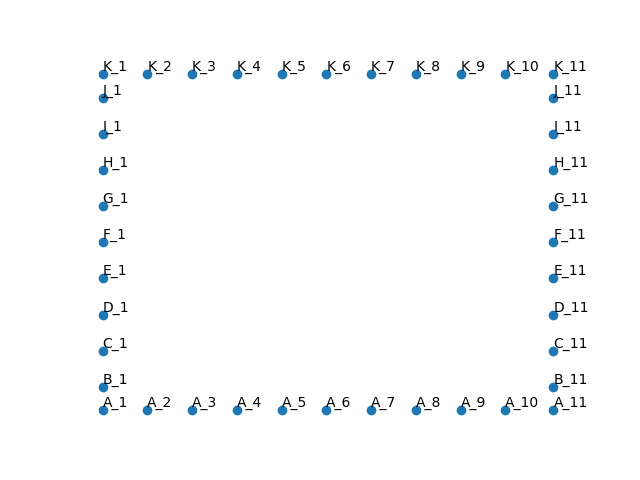
\includegraphics[width=0.7\textwidth]{assets/img/reperage_points_appuis.png} % Pour insérer l'image
    \caption{Repèrage des points d'appui 2D} % Légende de l'image
\end{figure}

\begin{figure}[H] % Pour insérer une figure
    \centering % Pour centrer l'image
    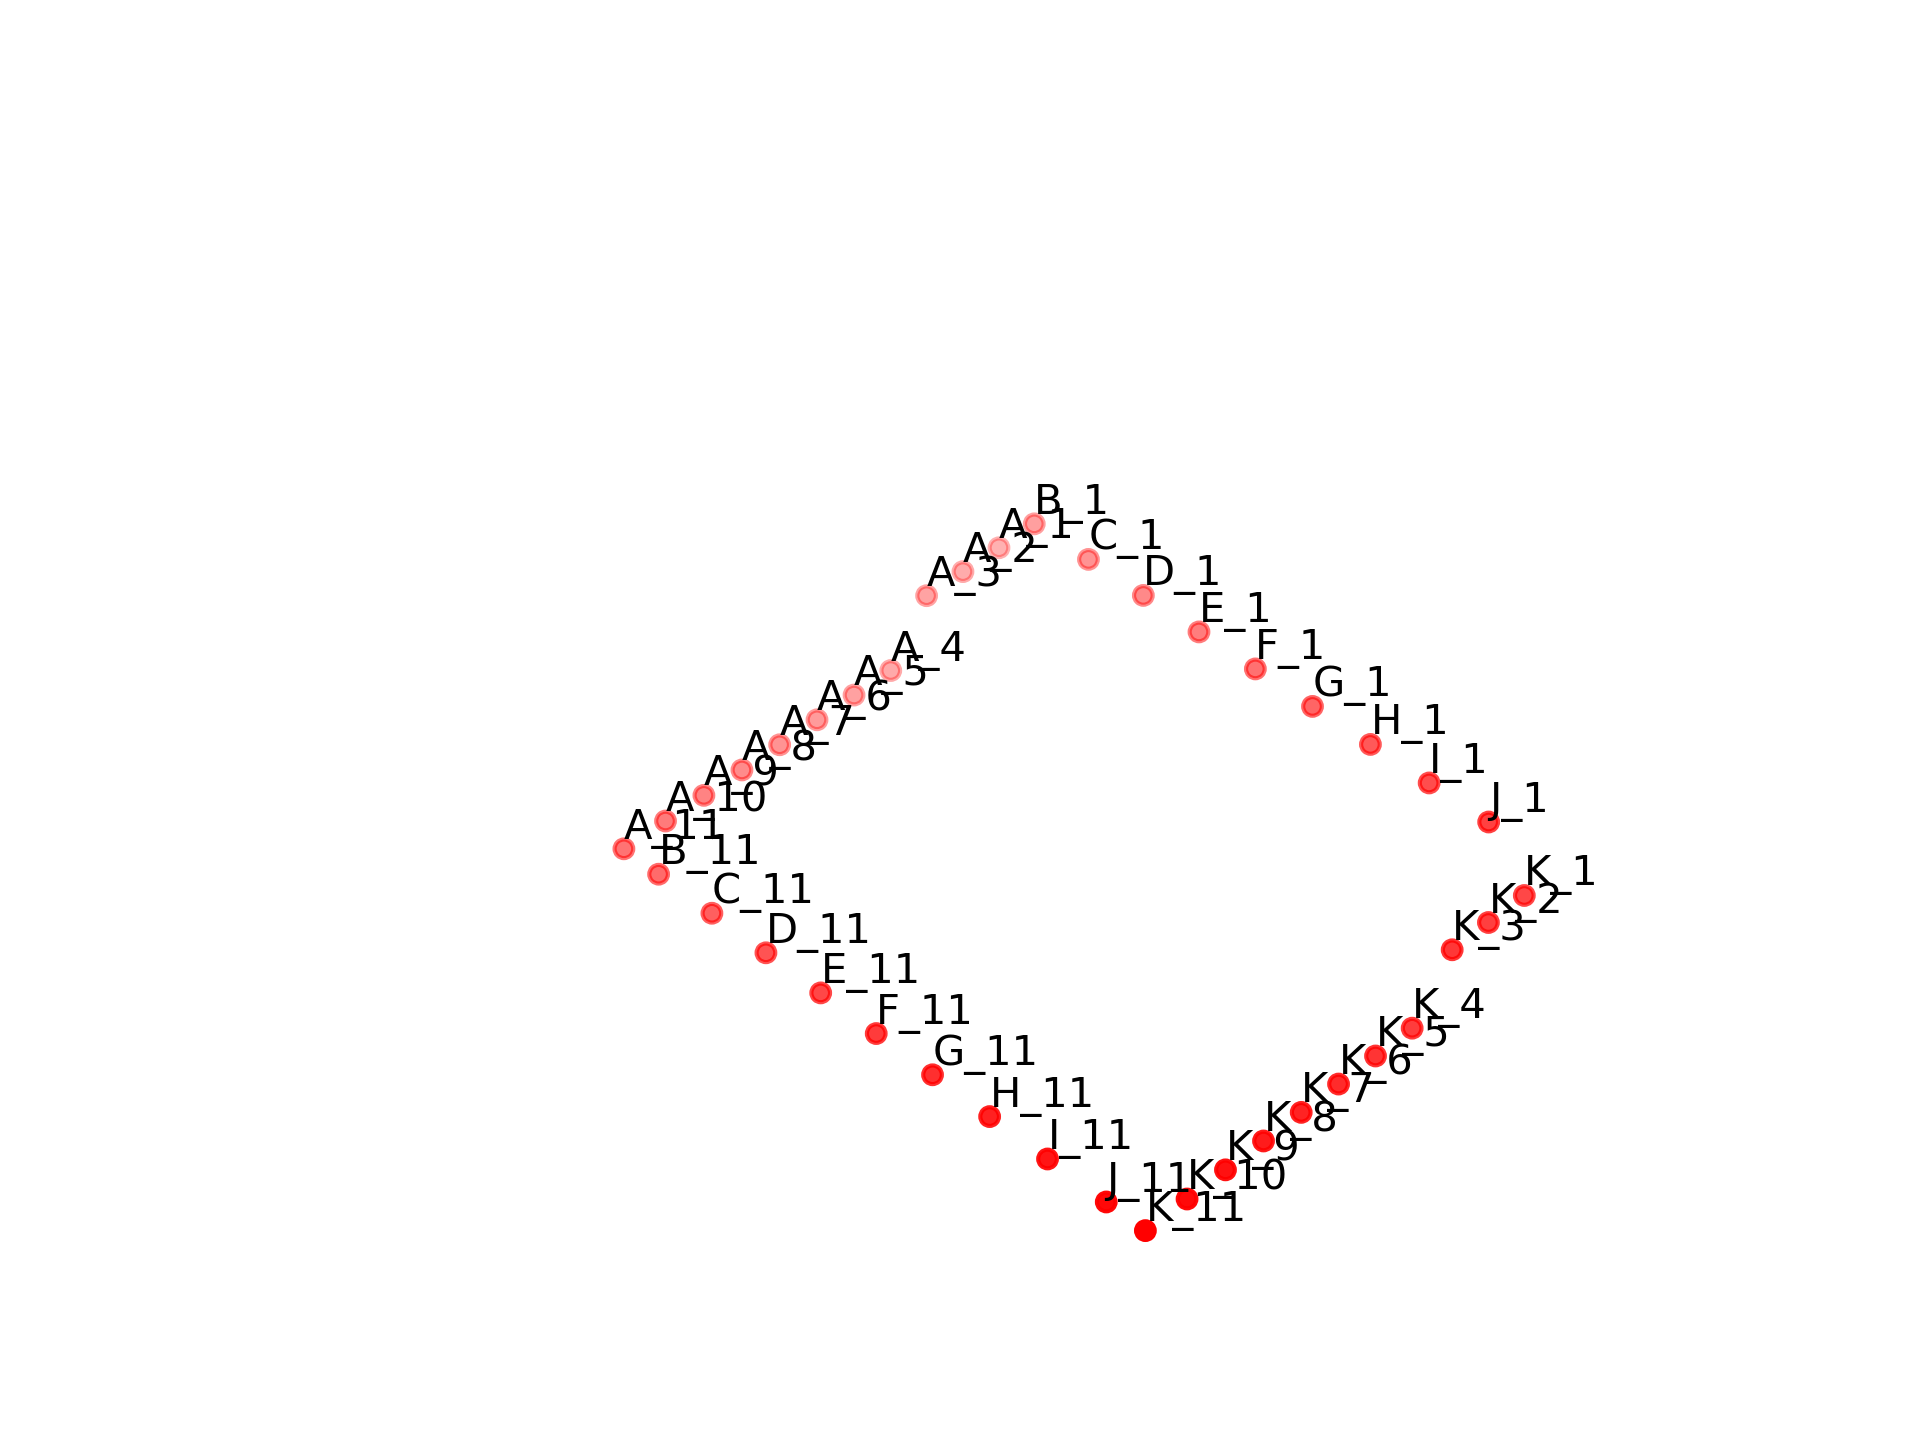
\includegraphics[width=\textwidth]{assets/img/reperage_points_appuis_3D_cas_1.png} % Pour insérer l'image
    \caption{Repèrage des points d'appui 3D} % Légende de l'image
\end{figure}



%%%%%%%%%%%%%%%%%%%%%%
%% DESCENTE DE CHARGES
%%%%%%%%%%%%%%%%%%%%%%

\import{latex_files/}{insert_nb_cas.tex}

%%%%%%%%%%%%%%%%%%%%%%
%% Tableaux et figure
%%%%%%%%%%%%%%%%%%%%%%
\newpage
{
    \markboth{}{Tableaux et figures}
    \phantomsection

    \listoffigures
    \addcontentsline{toc}{chapter}{\listfigurename}

    \listoftables
    \addcontentsline{toc}{chapter}{\listtablename}
}
\end{document}




































% Start the rest of the document
% Continue with the main content of your document



% \RPeda{{\sc SNOUSSI} Hichem} % Responsable pédagogique

% \Entreprise{SIMONIN} % Nom de l'entreprise / organisme / institution
% \Lieu{22 ZA des épinottes, 25500 Montlebon - France} % Adresse de l'entreprise
% \REntre{GAVIGNET Christian} % Responsable entreprise

% % Mots clés du Thésaurus ou mots clés pour les metadatas du pdf
% \Kone{Intelligence Artificielle, Détection d'objet} % Nature de l'activité
% \Ktwo{Construction bois, charpente, menuiserie} % Branche d'activité économique
% \Kthree{Bois lamellé-collé, isolation, bardage} % Domaines technologiques
% \Kfourth{Amélioration qualité} % Application directe
% %%%%%%%%%%%%%%%%%%%%%%%%%%%%%%%%%%%%%%%%%%%%%%%%%%%%%%%%%%%%

% %\Semestre{Année 2023-2024}
% \Semestre{2023-2024}
% %\UE{LT01} %Nom de l'UE OU nom complet de la branche si en mode rapport de stage !
% \UE{Mastère Spécialisé\textregistered{} EBDE}

% % Le titre de votre rapport OU le résumé de votre stage si en mode stage
% % \newcommand{\titletext}{Un rapport en \LaTeX \\ écrit avec amour}

% \newcommand{\titletext}{

%     Cette thèse professionnelle s'est déroulée dans l'entreprise Simonin. L'objectif était d'améliorer la qualité du tri 
%     du bois grâce à une solution d'Intelligence Artificielle intégrant la détection et le stockage de défauts de bois observés sur des planches.
%     Cette reconnaissance de défauts permettant ensuite d'apporter une aide au tri pour l'opérateur de production ainsi que des tableaux de bord qualité pour
%     le responsable production.

%     Les étapes réalisées:

%     \begin{itemize}
%         \item Analyse des besoins, définition de l'architecture de l'application et des données
%         \item Mise en place d'un système d'acquisition et d'annotation des images
%         \item Entrainement et évaluation du modèle
%         \item Stockage des résultats dans une base de données
%         \item Création d'une interface visuelle d'aide au tri et de synthèse qualité
%     \end{itemize}

%    L'enjeu est de développer pour cette PME une solution complète qui contribuera à une meilleure satisfaction du client ainsi 
%    qu'à une réduction des coûts.
% }



% %% En mode Année - Mois - Jour
% %\date{\today} % Pour la date de compilation
% \date{\today}

% \author{{\sc MORAND} Nicolas
% % \and
% % {\sc Nom} Prénom
% % \break
% % {\sc Nom} Prénom
% % \and
% % {\sc Nom} Prénom
% % \break
% % {\sc Nom} Prénom
% }

% % Texte affiché sur le carré bleu
% \newcommand{\jobposition}{}
% %\title{Vous êtes probablement assez bon pour travailler dans cette entreprise pour laquelle vous pensez ne pas être assez bon.}

% \title{Amélioration de la qualité du bois par reconnaissance et tri des défauts} 

% %%%%%%% Pour les métadonnées
% % Fonctionne, seulement il y a un warning à cause des "\\" dans le title
% % A tester ! Pour voir les infos du pdf on fait pdfinfo sous linux
% % https://ctan.gutenberg.eu.org/macros/latex/contrib/hyperref/doc/hyperref-doc.pdf#subsection.3.7
% \hypersetup{
%     pdfauthor = {\theauthor}, % Auteur : pdfauthor = {\theauthor}
%     pdftitle = {\thetitle}, % Titre : pdftitle = {Titre du document}
%     pdfkeywords = {Thèse professionnelle, \theKtwo, \theKthree, \theKfourth}
% }

% %%%%%%%
% % n'oubliez pas de changer le language principal dans rUTT.cls
% % en options du package babel !

% \begin{document}
% %%%% - Choix de la page de garde

% %\frontpagereports % Pour le modèle rapports de TDs / TPs / Projets
% \frontpageSTB % Pour le modèle rapports de Stages des Branches / Master
% %\frontpageSTC % Pour le modèle rapports de Stages des TC

% {
%     % \selectlanguage{english}
%     \myILB
% }

% % page blanche après page de garde pour impression recto verso

% \pagestyle{UTT} % Pour que notre document utilise ce style
% % Ici on organise nos parties
% \justifying % on justifie notre texte via ragged2e


% \pagenumbering{gobble} % on n'affiche pas les numéros de page
% \import{latex-files/}{remerciements.tex} % Toujours avant le sommaire !

% \clearpage

% %%%%%%%%%%%%%%%%%%%%%%
% %% Sommaire
% %%%%%%%%%%%%%%%%%%%%%%

% {
%     \setcounter{tocdepth}{1}
%     \renewcommand{\contentsname}{Sommaire}
%     \tableofcontents
% }

% \clearpage

% {
%     % Tableaux et figures
%     \markboth{}{Tableaux et figures}
%     \phantomsection

%     \listoffigures
%     \addcontentsline{toc}{chapter}{\listfigurename}

%     \listoftables
%     \addcontentsline{toc}{chapter}{\listtablename}
% }

% % \setglossarystyle{listhypergroup}
% % \printglossary[type=\acronymtype, title={Liste des acronymes}, toctitle={Liste des acronymes}]
% % \printglossary[title={Glossaire}, toctitle={Glossaire}]

% \clearpage


% \pagenumbering{arabic}

% \import{latex-files/}{introduction.tex}

% \clearpage

% \import{latex-files/}{presentation.tex}
% \import{latex-files/}{one.tex}
% \import{latex-files/}{two.tex}
% \import{latex-files/}{three.tex}
% \import{latex-files/}{four.tex}
% \clearpage

% \import{latex-files/}{conclusion.tex}
% \label{LastPage}

% \clearpage

% % Bibliographie !
% {
%     \pagenumbering{gobble} % On n'affiche pas les numéros de page
%     \phantomsection % hyperlinks will target the correct page
%     \markboth{Bibliographie}{}
%     \raggedright % pour éviter certaines erreurs rares d'affichage
%     \sloppy
%     \nocite{*} % pour faire apparaître tout du fichier bib
%     \printbibliography[title={Bibliographie},heading=bibintoc]
% }

% \clearpage

% %\tripleS
% \pagenumbering{Roman} % On numérote en romain pour les annexes

% % Annexes !
% \import{latex-files/annexes/}{annexes.tex}

% \clearpage
% % Toujours avoir la table des matières en dernier ! Ici figure tout, même les annexes
% % Commenter/supprimer pour enlever la table des matières
% \myfinaltoc
% % On laisse une page blanche à la fin pour l'impression, c'est plus joli
% \clearpage
% \myemptypage

\end{document}
